\documentclass[jocse]{jocseart}

\usepackage{booktabs}
\usepackage[utf8]{inputenc}
\usepackage[english]{babel}

% Copyright
\setcopyright{jocsecopyright}
\jocseDOI{10.22369/issn.2153-4136/x/x/x }

\pagestyle{plain}
\pagenumbering{gobble}

\usepackage{cleveref}
\usepackage{todonotes}
\usepackage{graphicx}
\graphicspath{{./fig/}}
\DeclareGraphicsExtensions{.png,.pdf,.jpg,.jpeg}

\newcommand{\jk}[1]{\todo[inline]{TODO: #1}}

\begin{document}
\title{Looking Back: One Year HPC Certification Forum}

\author{Julian Kunkel}
\affiliation{%
  \institution{University of Reading}
  \streetaddress{}
  \city{Reading}
  \state{United Kingdom}
  \postcode{}
}
\email{j.m.kunkel@reading.ac.uk}


\author{Kai Himstedt}
\author{Nathanael Hübbe}
\affiliation{%
  \institution{Universität Hamburg}
  \streetaddress{}
  \city{Hamburg}
  \state{Germany}
  \postcode{}
}

\author{Weronika Filinger}
\affiliation{%
  \institution{EPCC, The University of Edinburgh}
  \streetaddress{}
  \city{Edinburgh}
  \state{United Kingdom}
  \postcode{}
}

\author{Jean-Thomas Acquaviva}
\affiliation{%
  \institution{DDN}
  \streetaddress{}
  \city{Paris}
  \state{France}
  \postcode{}
}


\author{Anja Gerbes}
\affiliation{%
  \institution{Goethe-Universität}
  \streetaddress{}
  \city{Frankfurt am Main}
  \state{Germany}
  \postcode{}
}

\author{Lev Lafayette}
\affiliation{%
  \institution{University of Melbourne}
  \streetaddress{}
  \city{Melburne}
  \state{Australia}
  \postcode{}
}

\renewcommand{\shortauthors}{J. Kunkel et al.}


\begin{abstract}
  The HPC community has always considered the training of new and existing HPC practitioners to be of high importance to its growth.
  This diversification of HPC practitioners challenges the traditional training approaches, which are not able to satisfy the specific needs of users, often coming from non-traditionally HPC disciplines, and only interested in learning a particular set of competences.
  Challenges for HPC centres are to identify and overcome the gaps in users’ knowledge, while users struggle to identify relevant skills.

  With the HPC Certification Forum we aim to clearly categorize, define, and examine competences which brings benefit to all stakeholders involved in training.
  In this paper, we report the status and progress this independent body has made during the first year of its existence.
  Particularly, in various directions drafts of processes and prototypes have been generated to create a holistic ecosystem that will mature over this year.
\end{abstract}

%
% The code below should be generated by the tool at
% http://dl.acm.org/ccs.cfm
% Please copy and paste the code instead of the example below.
%
\begin{CCSXML}
\end{CCSXML}



\keywords{}

\maketitle

\section{Introduction}

There is a generally accepted set of skills and competencies necessary to efficiently use HPC resources.
This skill set depends on the role and domain of the practitioner but also on the available infrastructure of the center providing the computing resources.
For example, a scientist needing to run an application on a specific machine may need basic skills in Linux, MPI, environment modules, and knowledge about the batch scheduler, e.g., SLURM.
Understanding SLURM is a good example of a very fine-grained skill, indeed we can identify "resource management" as a generic skill that illustrates concepts across the rich variety of available resource managers.
Institutions which operate HPC systems typically offer regularly teaching events about general aspects of their supercomputer's hard- and software architecture and about the software environment around parallel programming and optimization.
The learning material provided by an HPC center, however, is geared to the special demands of the institutions they support and its specific HPC environment.
This content typically covers a small part of basic HPC skills which are necessary to use other HPC systems.
Moreover, they do not attest the users to have a certain competence.
Certificates are widely used in industry to attest certain knowledge but, so far, there is no similar approach for HPC training.

This article describes the current status of the certification program by looking back for the one year of this independent body that curate the competences and aims to issue certificates for the users.
Our previous work described the evolution from the project that sparked the initial activity that lead to the independent body of the HPC Certification forum \cite{TAHCPKHHSS19}.


\section{The HPC Certification Forum}

\section{Skill Organization}

\subsection{Skill Example}

\section{Certification}

\subsection{Certificates}

\subsection{Examination Process}

\section{Ecosystem}

\subsection{Linking Training Material}

\subsection{Supportive Tools}

\section{Discussion of the Benefits}

Making clear what skills are required of or recommended for a competent HPC user would benefit both the HPC service providers and practitioners.
Moreover, it would allow centres to bundle together skills that are most beneficial for specific user roles and scientific domains.
From the perspective of content providers, existing training material can be mapped to competences allowing users to quickly identify and learn the skills they require.
Finally, the certificates recognized by the whole HPC community simplify inter-comparison of independently offered courses and provide additional incentive for participation.


\section{Conclusion}



\begin{figure*}[tb!]
	\centering
	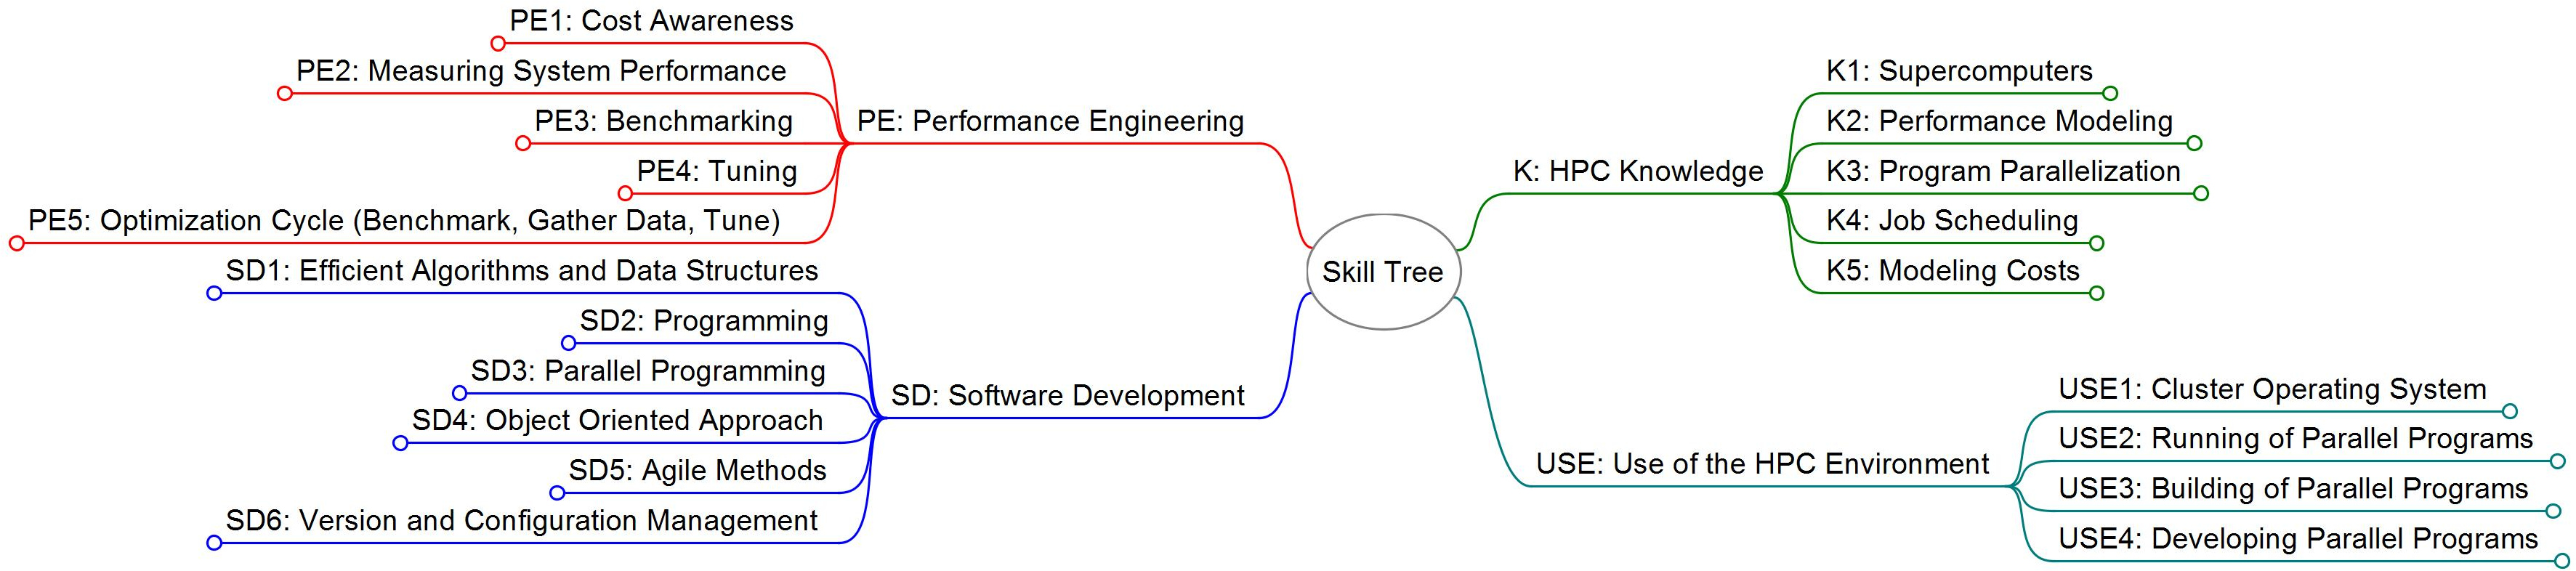
\includegraphics[width=15.0cm]{skill-tree_top_levels.jpg}
  \vspace*{-2em}
	\caption{Top Level Competences}
	\label{f_top_level_competences}
\end{figure*}

\section{Related Work}
\jk{Please everyone!}

Relevant work can be classified into approaches to establish a curriculum or the creation of teaching material.
In academia, individual universities offer their own curriculum around scientific computing and HPC, covering theoretical aspects like the software development of numerical applications.
They are not tailored to the needs of a practitioner to actually use HPC systems effectively.
Data centers offer their own material and courses to support their own users.
Several projects address the generation and sharing of teaching material for HPC.
The EuroLab-4-HPC project establishes training in form of (online) courses\footnote{\url{https://www.eurolab4hpc.eu/}}.
The Barcelona Supercomputing Centre (BSC) aims to develop a professional training curriculum \cite{sancho2016bsc}.
The virtual organization XSEDE\footnote{\url{https://portal.xsede.org/web/xup/training/overview}} provides an online system to train the usage of an HPC system, structuring the corresponding information on their website into major topics like “Getting Started”.
The user can navigate the topics and receive further information.






\section{Certification Program}

The certification program serves two purposes:
1) the definition and organization of fine-grained competences (skills);
2) the establishment of certificates and (online) exams that confirm that users possess a certain skill.
Note that the certification program does not regulate the content -- the definition of skills and certificates is separated from content creation.
This allows the re-use of existing content but also allows to create a new ecosystem in which HPC centers or commercial companies could offer the best teaching material.
Teaching material should be marked to indicated which skills it covers.
In the future, the program may provide means to register and reference existing content of third-parties allowing users to browse the skills and navigate to teaching material.
We assume that the collaboration of scientific institutions will complement each other in producing a rich variety of content for the different learning styles.


\subsection{Skills}

The skills represent competences in a fine-grained fashion.
A skill is defined by a unique key, short name, background, level, and a description of what it encompasses.
This model can be compared to the classification of school knowledge, for example, the skill with the short name "addition" could describe the math skill of being able to add numbers successfully.
The level serves the purpose of distinguishing the expertise further, a \textit{basic level}, for example, may mean to be able to add two numbers between 1-20 while the \textit{expert level} of that skill could indicate to be able to add any numbers.

The individual skills are organized into a tree that shows generic competences close to the root and refined skills on the leafs.
The two top-levels of the skill tree are shown in \Cref{f_top_level_competences}; we have identified more than 35 skills.
In respect to the granularity, we expect the basic level of a leaf like “Bash programming” can be acquired by novel users in a workshop day.
The tree serves the purpose of navigating across the skills, and at the same time a parent node defines the scope of its children.
For example, the \textit{USE} competence provides means of using the HPC environment to perform various tasks, such as running parallel applications, using core services of the operating system.
While the tree structure has been chosen as a graphical representation, some competences are cross-referenced, particularly in the skills of the USE branch.
The tree is managed in an XML file and we offer tools to visualize the skills as mindmap or embed them into a webpage.

\subsection{Certificates}

Certifying users with a certain competency is a core element of the program.
Since we identified so many skills, it is not useful to perform an exam on a single competence like “SLURM”.
Therefore, initially, we aim to group sets of skills into certificates and establish an online examination that attests users that they mastered a certain skill.
To be meaningful these tests must prevent cheating to some extent.
However, as any examination can be cheated with sufficient effort, we focus on practical aspects like a huge corpus of questions and some instantiated questions like \textit{how would you start ProgramX with 4 MPI processes?}

\section{Conclusions}

The HPC Certification program offers a strategy to classify and organize HPC competences.
While the idea started with the PeCoH project, we are supporting the HPC Certification Forum\footnote{\url{https://hpc-certification.org}} which is an independent international body that aims to sustain the work.
The certification forum has the role of a (virtual) central authority to curate and maintain the skill tree and certificates.
Moreover, the forum supports tools and an ecosystem around the competences.


\appendix

\begin{acks}
\small
This work was supported by the German Research Foundation (DFG) under grants LU 1353/12-1, OL 241/2-1, and RI 1068/7-1.
\end{acks}

\bibliographystyle{ACM-Reference-Format}
\bibliography{bibliography}

\end{document}
